% Straight up stealing preamble from Eli Holmes 
%%%%%%%%%%%%%%%%%%%%%%%%%%%%%%%%%%%%%%START PREAMBLE THAT IS THE SAME FOR ALL EXAMPLES
\documentclass{article}

%Required: You must have these
\usepackage{Sweave}
\usepackage{graphicx}
\usepackage{tabularx}
\usepackage{hyperref}
\usepackage{natbib}
\usepackage{pdflscape}
\usepackage{array}
\usepackage{gensymb}
\usepackage{authblk}
\renewcommand{\baselinestretch}{1.8}
\usepackage{lineno}
%\usepackage[backend=bibtex]{biblatex}
%Strongly recommended
 %put your figures in one place
 
%you'll want these for pretty captioning
\usepackage[small]{caption}

\setkeys{Gin}{width=0.8\textwidth} %make the figs 50 perc textwidth
\setlength{\captionmargin}{30pt}
\setlength{\abovecaptionskip}{0pt}
\setlength{\belowcaptionskip}{10pt}
\newcolumntype{L}[1]{>{\raggedright\let\newline\\
\arraybackslash\hspace{0pt}}m{#1}}
% manual for caption http://www.dd.chalmers.se/latex/Docs/PDF/caption.pdf

%Optional: I like to muck with my margins and spacing in ways that LaTeX frowns on
%Here's how to do that
 \topmargin -2cm 
 \oddsidemargin -0.04cm 
 \evensidemargin -0.04cm % same as oddsidemargin but for left-hand pages
 \textwidth 16.59cm
 \textheight 22.94cm 
 %\pagestyle{empty} % Uncomment if don't want page numbers
 \parskip 7.2pt % sets spacing between paragraphs
 %\renewcommand{\baselinestretch}{1.5} 	% Uncomment for 1.5 spacing between lines
\parindent 0pt% sets leading space for paragraphs
\usepackage{setspace}
%\doublespacing

%Optional: I like fancy headers
\usepackage{fancyhdr}
\pagestyle{fancy}
\fancyhead[LO]{Experimental climate change}
\fancyhead[RO]{2018}

%%%%%%%%%%%%%%%%%%%%%%%%%%%%%%%%%%%%%%END PREAMBLE THAT IS THE SAME FOR ALL EXAMPLES

%Start of the document
\begin{document}

% \SweaveOpts{concordance=TRUE}
\bibliographystyle{/Users/aileneettinger/citations/Bibtex/styles/ecol_let.bst}

\title{How do climate change experiments alter plot-scale climate?}
\author[1,2,a]{A.K. Ettinger}

\author[3,b]{I. Chuine}

\author[4,5,c]{B.I. Cook}

\author[6,d]{J.S. Dukes}

\author[7,e]{A.M. Ellison}

\author[8,f]{M.R. Johnston}

\author[9,g]{A.M. Panetta}

\author[10,h]{C.R. Rollinson}

\author[11,12,i]{Y. Vitasse}

\author[1,8,13,j]{E.M. Wolkovich}

\affil[1]{Arnold Arboretum of Harvard University, Boston, Massachusetts 02131, USA}

\affil[2]{Tufts University, Medford, Massachusetts 02155, USA}

\affil[3]{CEFE UMR 5175, CNRS, Universit\'e de Montpellier, Universit\'e Paul-Val\'ery Montpellier, EPHE IRD, Montpellier, France}

\affil[4]{Lamont-Doherty Earth Observatory, Columbia University, Palisades, New York 10964, USA}

\affil[5]{NASA Goddard Institute for Space Studies, New York, New York 10025, USA}

\affil[6]{Department of Forestry and Natural Resources
and Department of Biological Sciences, Purdue University, West Lafayette, Indiana 47907, USA}

\affil[7]{Harvard Forest, Harvard University, Petersham, Massachusetts 01366, USA}

\affil[8]{Department of Organismic and Evolutionary Biology, Harvard University, Cambridge, Massachusetts 02138, USA}

\affil[9]{Department of Ecology and Evolutionary Biology, University of Colorado, Boulder, Colorado 80309, USA}

\affil[10]{Center for Tree Science, The Morton Arboretum, Lisle, Illinois 60532, USA}

\affil[11]{Institute of Geography, University of Neuch\^atel, Neuch\^atel, Switzerland}

\affil[12]{Swiss Federal Institute for Forest, Snow and Landscape Research WSL, Neuch\^atel, Switzerland}

\affil[13]{Forest \& Conservation Sciences, Faculty of Forestry, University of British Columbia, Vancouver, BC, Canada}

\affil[a]{Corresponding author; email: aettinger@fas.harvard.edu; phone: 781-296-4821; mailing address: 1300 Centre Street, Boston, Massachusetts 02140, USA }

\affil[b]{isabelle.chuine@cefe.cnrs.fr}

\affil[c]{bc9z@ldeo.columbia.edu}

\affil[d]{jsdukes@purdue.edu}

\affil[e]{aellison@fas.harvard.edu}

\affil[f]{mjohnston@g.harvard.edu}

\affil[g]{anne.panetta@colorado.edu}

\affil[h]{crollinson@mortonarb.org}

\affil[i]{yann.vitasse@wsl.ch}

\affil[j]{e.wolkovich@ubc.ca}


\date{\today}
\maketitle %put the fancy title on
%\tableofcontents %add a table of contents

\textbf{Statement of authorship} %Statement of authorship: Contributions by authors should be listed on the title page and will be printed at the end of the manuscript. This statement should be appropriate to the study described in the manuscript and should clarify who designed the study, who performed the research, who provided new methods or materials, and who wrote the manuscript. We encourage concise statements such as ?JW performed phylogenetic analyses, MH collected data, performed modeling work and analyzed output data, and PK performed the meta-analysis. MH wrote the first draft of the manuscript, and all authors contributed substantially to revisions.?
All authors conceived of this manuscript, which was inspired by our discussions at a Radcliffe Exploratory Seminar in 2016, and all authors contributed to manuscript revisions. AKE and EMW conceived of the idea for the literature review, database compilation, and related Radcliffe Exploratory Seminar. AKE compiled the datasets; AKE and CRR analyzed the data and created the figures; AKE wrote the manuscript.

\textbf{Data Accessibility} %Data accessibility statement: The statement must confirm that, should the manuscript be accepted, the data supporting the results will be archived in an appropriate public repository such as Dryad or Figshare and the data DOI will be included at the end of the article.
The MC3E database will be available at KNB \citep{ettinger2018}, along with all R code from the analyses included in this paper. (Currently, metadata are published there; the full database and R code are available to reviewers on github.) 

\textbf{Running title} Experimental climate change

\textbf{Key words} global warming, warming experiment, microclimate, soil moisture, spring phenology, budburst, direct and indirect effects, structural control, hidden treatment, active-warming, target temperature, feedback

\textbf{Type of article} Review and Synthesis

\textbf{Number of words in abstract} 227

\textbf{Number of words in main text} 4,933%(excluding abstract, acknowledgements, references, table and figure legends), 

\textbf{Number of references} 97

\textbf{Number of figures} 6

\textbf{Number of tables} 1

\textbf{Number of text boxes} 2

\textbf{Number of words in Box 1} 482

\textbf{Number of words in Box 2} 570

\clearpage

\clearpage
%%%%%%%%%%%%%%%%%%%%%%%%%%%%%%%%%%%%%%%%%%%%%%%%%%%
\linenumbers



\section*{Abstract}
\par To understand and forecast biological responses to climate change, scientists frequently use field experiments that alter temperature and precipitation. Climate manipulations can manifest in complex ways, however, challenging interpretations of biological responses. We reviewed publications from active-warming experiments to compile a database of daily plot-scale climate data from 15 experiments that use forced air, infrared heaters, or soil cables to warm plots. We find that the common practices of analyzing primarily mean changes among treatments and analyzing treatments as categorical variables (e.g., warmed verses unwarmed) masks important variation in treatment effects over space and time. Our synthesis showed that measured mean warming, in plots with the same target warming, differed by 1.6\degree C, on average, with high variation---maximum differences ranged from 0.03 - 4.87\degree C across studies, which varied in warming design and myriad ecosystem attributes. Warming treatments produce non-temperature effects as well, such as soil drying. The combination of these direct and indirect effects is complex and can have important biological consequences. With a case study of plant phenology, we show how accounting for drier soils with warming triples the estimated sensitivity of budburst to temperature. Our synthesis yields recommendations for future analyses, experimental design, and data sharing to improve our mechanistic understanding of what drives variation across studies, and thus improve the utility of climate change experiments to accurately identify and forecast species' responses.


 
\section* {Introduction}
\par Climate change is dramatically altering earth's biota, shifting the physiology, distribution, and abundance of organisms, with cascading community, ecosystem, and climate effects \citep{shukla1982,cox2000,thomas2004,parmesan2006,field2007,sheldon2011,urban2012}. Much uncertainty exists about how particular individuals, populations, species, communities, and ecosystems will respond as warming becomes more extreme \citep{thuiller2004,friedlingstein2014}.
Predicting biological responses to current and future climate change---and their feedbacks to earth's climate and ecosystem services---is one of the most significant challenges facing ecologists today.
\par Two common approaches for understanding biological effects of climate change are observational studies, which correlate recorded biological patterns with measured climate, and process-based modeling; yet these approaches are insufficient for several reasons. 
Observational studies and correlative models cannot disentangle the causal effects of warming (one aspect of climate) from other factors that have also changed over time, such as successional stage or land use. In addition, models based on correlative data may fail to make useful predictions for future conditions that fall outside the range of historical variability \citep [e.g.,][]{pearson2004,hampe2004,ibanez2006,swab2012,chuine2016}. Climate change will yield warmer temperatures than the previous 150 years, and possibly warmer than at any time in the last 2000 years \citep{ohlemuller2006,williams2007,williams2007b,ipcc2013}. Process-based models overcome some of these challenges through inclusion of explicit mechanistic relationships between climate and biological outcomes. However, they are limited by the processes they include (i.e., our understanding of mechanism), as well as by the data available to parameterize those processes \citep{moorcroft2006,kearney2009}. 

\par Experimental data from field-based climate change experiments are crucial to fill these knowledge gaps and determine mechanistic links between climate change and biological responses. Experiments can quantify biological responses to different levels of climate change, and can create the ``no-analog" climate scenarios forecasted for the future, particularly when they employ active-warming methods, such as forced air heaters, soil warming cables, or infrared heaters \citep{shaver2000,williams2007b,aronson2009}. In addition, active-warming can be combined with precipitation manipulations (e.g., snow removal, water additions or reductions), offering the ability to assess individual and interactive effects of temperature and precipitation, separate from other environmental changes \citep [e.g.,][]{price1998,cleland2006,sherry2007,rollinson2012}. Compared with indoor growth-chamber experiments, field-based experiments offer the possibility of preserving important but unknown or unquantified feedbacks among biotic and abiotic components of the studied systems. %CRR: Do we need to elaborate here? If so maybe an example about warming effects on nitrogen mineralization or something along those lines? Looks like Charles & Dukes 2009 Ecol Apps ("Effects of warming and altered precipitation on plant and nutrient dynamics of a New England salt marsh."); and Heskel et al 2014 GCB ("Thermal acclimation of shoot respiration...") might be appropriate.

\par With climate change experiments, ecologists often aim to test hypotheses about how projected warming will affect species' growth, survival, and future distributions \citep{dukes1999,hobbie1999,morin2010,pelini2011,chuine2012,reich2015,gruner2017}. %But is it reasonable to extrapolate findings from these experiments to the real world? In what ways is plot-level climate altered by climate manipulations? %How can we more fully utilize experimental data to improve understanding of the mechanisms behind observed biological response to climate manipulations? 
Recent research suggests, however, that climate manipulations may not always alter plot-scale climate (hereafter, microclimate) in ways that are consistent with observed changes over time \citep{wolkovich2012,menke2014,polgar2014,andresen2016}. For extrapolation of experimental findings to the real world, we need detailed assessments of how active-warming experiments alter the microclimate conditions experienced by organisms, and the extent to which these conditions are similar to current field conditions or anticipated climate change. 
\par Here, we investigate the complex ways that active-warming treatments alter microclimate, both directly and indirectly, across multiple studies. The qualitative challenges and opportunities of climate change experiments have been summarized previously \citep[e.g.,][]{deboeck2015} and effects of these manipulations on some aspects of microclimate have been published for individual sites \citep[e.g.,][]{harte1995b,mcdaniel2014,pelini2011}. However, our quantitative meta-analysis allows us to examine trends across sites and warming designs (Box 1, Table \ref{tab:warmtech}), and make recommendations based on this information. Using plot-level daily microclimate data from 15 active-warming experiments (yielding 59 experiment years and 14,913 experiment days; Table S1), we show the direct and indirect ways that experimental manipulations alter microclimate. We use a case study of spring plant phenology to demonstrate how analyses that assume a constant warming effect and do not include non-temperature effects of warming treatments on biological responses lead to inaccurate quantification of plant sensitivity to temperature shifts. Finally, we synthesize our findings to make recommendations for future analysis and design of climate change experiments (Box 2). 

\section* {MicroClimate from Climate Change Experiments (MC3E) database}
\par To investigate how climate change experiments alter microclimate, we first identified published, active-warming field experiments, many of which included precipitation manipulations. We focused on \textit{in situ} active-warming manipulations because recent analyses indicate that active-warming methods are the most controlled and consistent methods available for experimental warming \citep{kimball2005,kimball2008,aronson2009,wolkovich2012}. We do not include passive-warming experiments because they have been analyzed extensively already and are known to have distinct issues, including reduction in wind, overheating, and great variation in the amount of warming depending on irradiance and snow depth \citep[][see also Table S2]{marion1997,shaver2000,wolkovich2012,bokhorst2013}.
\par We carried out a full literature review to identify potential active-warming field experiments to include in the database. We followed the methods and search terms of \citet{wolkovich2012} for their Synthesis of Timings Observed in iNcrease Experiments (STONE) database \citep{wolkovich2012}, but restricted our focus to active-warming experiments. Further, because our goal was to tease out variation in microclimate (including temperature and soil moisture), we focused on warming studies that included both/either multiple levels of warming and/or precipitation treatments. These additional restrictions constrained the list to 11 new studies published after the STONE database, as well as six of the 37 studies in the STONE database. We contacted authors to obtain daily microclimate and phenological data for these 17 studies and received data (or obtained publicly available data) for 10 of them, as well as datasets from five additional sites offered or suggested to us over the course of our literature review and data analysis. The daily temperature and soil moisture data from these 15 experiments comprise the MicroClimate from Climate Change Experiments (MC3E) database (Figures \ref{fig:effwarm} and S1, Table S1), which is available at KNB \citep{ettinger2018}. We examined how these experiments altered microclimate, using mixed-effects models that allowed for inherent differences among studies (through a random effect of study on the intercept), while also estimating various across-study effects, such as degree of warming or warming type. 

\section* {Complexities in interpreting experimental climate change} 
Climate change experiments often include detailed monitoring of climate variables at the plot-level, yielding large amounts of data, such as daily or hourly temperature and other climate variables, over the course of an experiment. Ecologists, however, are generally interested in the ecological responses (e.g., community dynamics, species' growth, abundance, or phenology), which are collected on much coarser timescales (e.g., seasonally or annually). Not surprisingly then, when analyzing ecological responses, authors typically provide detailed information on the observed biological responses, and report only the mean change in climate over the course of the experiment and whether it matched their target level of change \citep[e.g.,][]{price1998,rollinson2012,clark2014a,clark2014b}. Several studies have conducted detailed, independent analyses of microclimate data from warming experiments \citep[e.g.,][]{harte1995b,kimball2005,kimball2008,mcdaniel2014, pelini2011}. While these detailed analyses provide valuable case studies of experimental effects on microclimate data alone, they have generally not been incorporated into analyses of ecological responses. 

\par In interpreting ecological responses to climate change manipulations, the focus has been primarily on mean shifts in microclimate, but the imposed manipulations result in much more complex shifts. The magnitude of change in these manipulations varies in time and space, and the presence of experimental equipment alone (with no heat added) often alters environmental conditions. These factors, discussed below, challenge our interpretation of how experimental warming studies forecast effects of climate change on organisms and ecosystems. When possible, we compare and contrast these factors across different study methodologies, such as infrared warming versus forced air chambers and constant wattage versus feedback control, because effects on microclimate may vary across these different methodologies (Box 1, Figure \ref{fig:exps}).

\subsection* {Effects on microclimate vary over time and space}
Reporting only the mean temperature difference across the duration of a warming study masks potentially important temporal variation in temperature among treatments (compare Figure \ref{fig:blockyear} to Figure S2). Using the MC3E database, we found that active-warming reduces the range of above-ground daily temperature by 0.37\degree C per \degree C of target warming (Table S3, see also Table S1, which details the different methods used to measure and warm temperatures). Active-warming decreased above-ground daily temperature range by differentially affecting maximum and minimum temperatures: warming increased daily minima by 0.81\degree C per \degree C of target warming, but only increased daily maxima by 0.48\degree C per \degree C of target warming (Table S3). These effects varied by site (Table S3), but we found no clear patterns by warming type (e.g., infrared versus forced air) or warming control (feedback versus constant). Soil daily temperature range was not affected by experimental warming, as warming altered minimum and maximum daily temperatures similarly (Table S4).

\par We observed strong seasonal and annual variations in the effects of experimental warming (Figures \ref{fig:effwarm}, \ref{fig:blockyear}, Table S5). Warming generally appears close to targets in winter and early spring, and farthest below targets in summer (day of year 150-200, when evapotranspiration within a robust plant canopy can dissipate energy and act to cool vegetation surfaces), though patterns differ among sites (Figure \ref{fig:effwarm}). 
The variation in warming effectiveness may be driven by interactions between warming treatments and daily, seasonal, and annual weather patterns, since the magnitude of warming can vary as weather conditions change. Both infrared heaters and soil cables fail to achieve target temperature increases during rainstorms \citep{peterjohn1993,hoeppner2012} and with windy conditions \citep{kimball2005,kimball2008}. Differences between target and actual warming are likely to be particularly great for studies employing constant wattage, rather than feedback control (Box 1, Figure 2). In addition, treatments are often applied inconsistently within or across years. Heat applications are frequently shut off during winter months, and some heating methods, even if left on throughout the year, do not warm consistently \citep[e.g.,][]{clark2014a,clark2014b,hagedorn2010}.

\par Treatment effects also vary spatially, further complicating interpretation of climate change experiments. The MC3E database contains six studies that used blocked designs, allowing us to examine spatial variation in the amount of warming (i.e., the difference between treatment and control plots within a block). These studies include two infrared with feedback control, three infrared with constant wattage, and one soil warming cable with feedback control experiments. We found that the amount of observed warming frequently varied by more than 1\degree C (mean= 1.6\degree C, maximum = 4.9\degree C) among blocks (Figure \ref{fig:blockyear}, Table S6). This variation in warming is substantial, as it is equivalent to the target warming treatment for many studies, and appears to vary substantially among sites, which differ in warming methodologies and environmental characteristics, though low sample sizes make disentangling the effect of warming method difficult (Box 1). The differences in warming among blocks may be caused by fine-scale variation in vegetation, slope, aspect, soil type, or other factors that can alter wind or soil moisture, which in turn affect warming \citep{peterjohn1993,kimball2005,kimball2008,hoeppner2012,rollinson2015}. %CRR: Also worth noting consistently increased variance in both control and treatments in the summer (Figures \ref{fig:effwarm})? To me this would highlight the role plant community dynamics can play in this since (I think) all of our plant communities are by and large seasonal/deciduous.. 


\par Of course, identical experimental treatments across space and time are neither necessary, nor realistic, for robust analysis of experimental results and forecasting. % Aaron: Are experimental data ever used in forecasting models? We did in some of our papers from the HF ant warming experiment, but I don't know how other models have used experimental data. Add Pecan ref here?
Indeed, the spatial and temporal variation we report could improve and refine models, and---at least in some regions---may be consistent with contemporary patterns of climate change \citep{ipcc2013}. Taking advantage of this variation, though, requires understanding and reporting it \citep[e.g.,][]{milcu2016}. However, because fine-scale and temporal variations in warming treatments are rarely analyzed explicitly with ecological data, the implications for interpretation of experimental findings are unclear.


\subsection* {Experimental infrastructure alters microclimate}
Experimental structures themselves can alter temperature and other important biotic and abiotic variables in ways that are not generally examined in experimental climate change studies. The importance of controls that mimic a treatment procedure without actually applying the treatment is widely acknowledged in biology \citep[e.g.,][]{dayton1971,spector2001,johnson2002,quinn2002}. Though some experimental climate change studies include treatments with non-functional warming equipment as well as ambient controls, the magnitude and effects of experimental infrastructure alone on climate are rarely interpreted or analyzed.
\par To investigate the magnitude of infrastructure effects, we compared temperature and soil moisture data from five active-warming studies at two sites: Duke Forest and Harvard Forest \citep{farnsworth1995,clark2014b, marchin2015, pelini2011}(see Supplemental Materials for model details). These were the only studies in the MC3E database that monitored climate in two types of control plots: structural controls (i.e., `shams' or `disturbance controls,' which contained the warming infrastructure: soil cables (n=1), forced air chambers (n=2), or both (n=2), but with no heat applied) and ambient controls with no infrastructure added. Other studies monitored environmental conditions in only structural controls (n=4) or ambient controls (n=5). We were unable to compare ambient and structural controls for experiments using infrared heating, because no studies in our database included both control types. A separate analysis suggested that there may be infrastructure effects on microclimate for infrared studies in our database (see Supplemental Materials, especially Table S7), and infrastructure effects have been documented in other studies \citep[e.g., shading][]{kimball2008}. 

\par We found that experimental structures altered above-ground and soil temperatures in opposing ways: above-ground temperatures were higher in the structural controls than in ambient controls, whereas soil temperatures were lower in structural controls compared with ambient controls (Figure \ref{fig:shamamb}a-d). This general pattern was consistent across different temperature models (mean, minimum, and maximum temperatures), although the magnitude varied among seasons, studies, and years (Figure \ref{fig:shamamb}a-d, Tables S8-S11). We also found that experimental infrastructure decreased soil moisture relative to ambient conditions across all seasons, studies, and years (Figure \ref{fig:shamamb}e, Tables S12, S13). 
\par There are several possible reasons for the observed climatic differences between ambient and structural controls. Infrastructure materials may shade the plots, reduce airflow, reduce albedo relative to surroundings, or otherwise change the energy balance, particularly in chamber warming (i.e., 4 of the 5 studies included in the above analysis). Specifically, soil temperatures may be cooler in structural controls for forced air studies because the experimental structures block sunlight from hitting the ground surface, causing less radiative heating of the ground in structural controls compared to ambient controls. In addition, above-ground temperatures may be warmer in structural controls because the structures radiatively warm the air around them and block wind, inhibiting mixing with air outside of the plot. Structures may also interfere with precipitation hitting the ground, thereby reducing local soil moisture and snowpack, with its insulative properties. These effects may be most dramatic in studies that employ chambers, rather than open-air designs, such as infrared heating \citep{aronson2009}. Finally, for some warming types (e.g., soil cables), structural controls experience increased soil disturbance compared with ambient controls; this may alter water flow and percolation, and introduce conductive material via the cables or posts. 

\par To the extent that differences between ambient and structural controls have been reported in previous studies, our findings appear to be consistent. Clark \textit{et al.} (2014b), who used forced air and soil cables with feedback control for warming, state that ``control of the air temperature was less precise, in part due to air scooping on windy days." Marchin \textit{et al.} (2015), who used forced air warming with feedback control, note that structural controls had mean spring air temperatures about 0.5\degree C or more above ambient temperatures. Peterjohn \textit{et al.} (1994), who warmed soil with heating cables and feedback control, reported cooler soil temperatures in structural controls than in ambient controls at shallow soil depths. Similarly, we found the greatest difference in soil temperature between structural and ambient controls in shallow soils (e.g., exp10, in which soil temperature was measured at a depth of 2cm). If addressed, the focus to date has been largely on these abiotic impacts of experimental structures, but structures may also alter herbivory and other biotic conditions \citep{kennedy1995,moise2010,wolkovich2012,hoeppner2012}. 

\par Our analyses suggest that warming experiments that calculate focal response variables relative to ambient controls \citep[e.g.,][]{price1998,dunne2003,cleland2006,morin2010,marchin2015} may not adequately account for the ways in which infrastructure affects microclimate. Results from studies reporting only structural controls \citep [e.g.,][]{sherry2007,hoeppner2012, rollinson2012}, should be cautiously applied outside of an experimental context, as---without ambient controls---their inference is technically limited to the environment of the structural controls. Our results suggest that studies aiming to predict or forecast the effects of climate change on organisms and ecosystems would benefit from employing both structural and ambient controls so that they may separate artifacts due to infrastructure from the effects of experimental warming. Increased use of both structural and ambient controls together would also help answer important questions of how infrastructure effects vary across ecosystem types, and warming designs (Box 1). 
\section* {Indirect and feedback effects of climate change manipulations} 
Climate change experiments often seek to manipulate temperature or precipitation separately as well as interactively. Manipulating either of these variables in isolation is notoriously difficult. Treatments involving precipitation additions typically reduce temperatures in climate change manipulations \citep{sherry2007,rollinson2012,mcdaniel2014}. For example, Sherry \emph{et al.} (2007) observed that a doubling of precipitation reduced mean air temperatures by 0.44\degree C, on average, during their one-year observation period. 
\par In the MC3E database, there are four experiments that manipulated both temperature and precipitation, and provided daily above-ground temperature data (three of these also measured soil temperature). Across these studies, all of which used infrared heating (two with feedback control and one with constant warming), we found that increasing the amount of added precipitation reduced daily minimum and maximum above-ground temperatures, at rates of 0.01 and 0.02\degree C, respectively, and soil temperatures, at a rate of 0.01\degree C for both minimum and maximum temperature, per percent increase in added precipitation (Table S14). Thus, a 50\% increase in precipitation would be expected to decrease temperature by 0.5\degree C.
This is likely because increasing soil moisture (an effect of precipitation additions) typically shifts the surface energy balance to favor latent (i.e., evapotranspiration) over sensible energy fluxes, reducing heating of the air overlying the soils. Maintaining target warming levels is a challenge even for independent feedback systems, which vary energy inputs using ongoing temperature measurements, particularly during seasons or years with wetter soils and higher evapotranspiration \citep{rich2015}.
\par In addition to its effects on temperature, experimental warming often increases vapor pressure deficit and reduces soil water content \citep[e.g.,][]{harte1995b,sherry2007,morin2010,pelini2014,templer2016}. Of the 15 experiments in the MC3E database, we examined the 12 that continuously measured and reported soil moisture. We included target warming, warming type, and their interaction as predictors (excluding data from plots with precipitation treatments) and accounted for other differences among studies by including a random effect of study (see Supplemental Materials for details). We found that experimental warming reduced soil moisture across all warming types, with substantial variation among experiments (Figure 5, Table S15). The drying effect varied by warming type (-0.80\% for infrared versus -0.33\% for forced air, per \degree C of target warming, Table S16). Soil moisture can be difficult to measure, with high spatial and temporal variation \citep{famiglietti1999,teuling2005}, but these results highlight that changes in soil moisture often accompany temperature changes in active-warming experiments.

\par Warming and precipitation treatments, and their indirect effects on soil moisture and other abiotic factors, can also alter the biotic environment, which may produce cascading effects. Many studies have found shifts from herbaceous to woody plant communities over time with experimental warming \citep[e.g.,][]{rollinson2012, mcdaniel2014,mcdaniel2014b, harte2015}. These community shifts may affect resource levels, such as moisture, carbon, and nutrient levels in the soil \citep{mcdaniel2014,mcdaniel2014b, harte2015} and feed back to affect microclimate \citep{harte2015}. 
\par The presence of these feedback effects is both a strength of and a challenge for climate change experiments. They may represent important and ecologically realistic effects that became apparent only with the \emph{in situ} field experiment. Alternatively, they may represent artifacts that are unlikely to occur outside of an experimental context. Quantifying, interpreting, and reporting these non-temperature effects in experiments is critical to distinguish these possibilities and to understand mechanisms underlying observed biological responses to climate change. 

\par The widespread presence of indirect effects of climate manipulations highlights the importance of measuring environmental conditions at the plot-level, and using these measurements in analysis and interpretation of results. Many papers published on climate change experiments---including 10 of the 15 references listed in Table S1---analyze warming and/or precipitation treatments as simple categorical predictors (e.g., as in a two-way ANOVA). Our findings, however, demonstrate a need for alternative modelling approaches to fully understand the experimental results and to make mechanistic links between changes in climate and ecological responses. One straightforward alternative is to include the continuous climate data (e.g., plot-level temperatures) as predictors of the focal response variable, such as phenological state or species density \citep [e.g.,][]{marchin2015, pelini2014}.
\section* {Ecological implications}

\par We have highlighted a suite of factors that complicate interpretation of climate change experiments. These indirect effects are likely to have biological implications for many of the responses studied in warming experiments (e.g., Figure \ref{fig:biolimp}). Interpretation of experimental climate change effects on biological responses may be misleading because the intended climate treatments (i.e., categorical comparisons or target warming levels) are often used as explanatory variables in analyses (Table S1). The interpretation is likely to be altered by using fine-scale, measured climate as explanatory variables. For example, biological responses may be muted (Figure \ref{fig:biolimp}b) or exaggerated (Figure \ref{fig:biolimp}c) when direct and indirect effects of climate manipulations interact.

\par To investigate the ecological implications of non-target abiotic responses to climate warming, we used a simple case study of plant phenology. We used the MC3E database to test if estimates of the temperature sensitivity of phenology vary when calculated using target warming versus plot-level climate variables. We fit two separate mixed-effects models, which differed in their explanatory variables: one used target warming and one used measured climate. Both models had budburst day of year as the response variable, and both included random effects of study (which modeled other differences between studies that may have affected phenology), year (nested within study, which modeled differences due to weather variability among years that may have altered phenology), and species (which often vary in their phenology). All random effects were modeled on the intercept only; see Supplemental Materials for details.

\par We found that phenological sensitivities to temperature estimated from the two modeling approaches varied three-fold. The target warming model estimated temperature sensitivity of budburst to be -1.91 days/\degree C (95\% CI -2.17, -1.86; Table S17, solid black line in Figure \ref{fig:phen}), whereas the measured climate model estimated temperature sensitivity of budburst to be -6.00 days/\degree C (95\% CI: -6.74, -5.26; Table S17). Further, all measured climate models with both temperature and moisture had improved model fit compared to the target warming model (Table S18). The best-fit model included mean daily minimum above-ground temperature, mean winter soil moisture, and their interaction as explanatory variables, suggesting that these variables are important drivers of budburst timing (Tables S17, S18). 
In addition, the measured climate model estimated a significant effect of soil moisture on budburst of -1.51 days/\% VWC (95\% CI: -1.76, -1.26; Table S17, Figure \ref{fig:phen}). This negative effect is expected, if reducing moisture delays budburst (Table S17, Figure \ref{fig:phen}), and is consistent with previous work showing that budburst requires water uptake \citep{essiamah1986}. 

\par The increase in estimated temperature sensitivity with measured (rather than target) temperature has two major causes. First, plot-level warming often does not reach target levels (Figure \ref{fig:blockyear}), producing a muted effect of temperature in models using target warming. Second, experimental warming's dual effects of decreasing soil moisture and increasing temperature impact budburst in contrasting ways. 
Decreasing soil moisture has a delaying effect on budburst phenology, opposing the advancing effect of rising temperatures (Figure \ref{fig:biolimp}b); thus the effect of temperature is underestimated when moisture is not included in the model. This example shows how the common method of using target warming alone, or even measured temperature alone as done in previous analyses of the particular experiments included here \citep[exp01, exp03, exp04, exp10,][]{clark2014a,clark2014b,polgar2014,marchin2015}, to understand biological responses may yield inaccurate estimates of temperature sensitivity in warming experiments. In this case, the underestimation may be substantial enough to account for previously described discrepancies between phenological responses to warming in observational versus experimental studies \citep{wolkovich2012,polgar2014}, though further investigation is required. 

\par Accounting for both direct and indirect effects of warming is critical for accurate interpretation of the consequences of climate change \citep{kharouba2015}. Of particular importance is the extent to which abiotic and biotic effects are realistic forecasts of future shifts that are likely to occur with climate change, or due to artifacts that are unlikely to occur outside of experimental systems \citep{hurlbert1984,moise2010,diamond2013}. For many important climatic and ecological metrics, experimental findings of abiotic and biotic effects appear to be consistent with observations. Altered above-ground daily temperature range (i.e., temperature minima changing more than maxima, Table S3) with experimental warming is consistent with observed changes in many places. Global minimum temperatures increased more rapidly than maximum temperatures from 1950-1980, reducing above-ground daily temperature range \citep[][]{thorne2016,vose2005}. In addition, the acclimation response of leaf respiration to temperature \citep{aspinwall2016,reich2016}, responses of soil respiration to warming \citep{carey2016}, and declines in soil carbon at one site \citep{harte2015}, also appear to be consistent across experiments and observations. These cases suggest that many responses observed in climate change experiments,including indirect effects of treatments, may be accurate harbingers of future biological responses to climate change. 

\par In contrast, some responses documented in climate change experiments may not be in line with future climate change---or may be too uncertain for robust prediction, and thus need explicit analyses and cautious interpretation. Although surface warming inevitably increases soil water evaporation, it does not necessarily translate to a decrease in soil water content. Precipitation forecasts with climate change are more uncertain than temperature forecasts, as are, consequently, future changes in soil moisture \citep{cook2018}. For example, soil drying is forecasted in some regions, such as the southwestern United States, mainly because of reductions in precipitation and increased evaporative demand associated with warmer air \citep{dai2013,seager2013}. The northeastern United States, on the other hand, has been trending wetter over time \citep{shuman2017}, even though temperatures have warmed. Shifts in soil moisture are likely to vary by region, season, vegetation type, and soil depth \citep{seager2014,berg2017,cook2018}. The uncertainty associated with forecasting changes to soil moisture makes replicating future water availability regimes in climate change experiments especially challenging; one way to meet this challenge and make predictions---even given high uncertainty---is to quantify soil moisture effects in climate change experiments. The altered light, wind, and herbivory patterns documented under experimental infrastructure \citep{kennedy1995,moise2010,wolkovich2012,hoeppner2012, clark2014b} represent other non-temperature effects that may be potential experimental artifacts and are worth quantifying in future analyses to provide improved estimates of temperature sensitivity.
\par An additional challenge in relating experiments to observations is that experimental findings may not scale up in space and time. Short-term responses to climate change frequently differ from long-term responses \citep{woodward1992,elmendorf2012, andresen2016, reich2018}. Differences may be, in part, because many experiments typically impose some mean shift in climate, but patterns of climate change are likely to be more variable. Many climate models project complex shifts in precipitation: more intense extreme precipitation events (e.g., heavy downpours), more dry days (i.e., less total precipitation events), or both \citep{polade2014}. In addition, the small spatial scale of experiments may result in responses that are unlikely to be observed at larger scales \citep{woodward1992,menke2014}. Experimental plots range in area from 1.5 to 36 square meters (Table S1), which may be too small to encapsulate, for example, the rooting zones of perennial plants \citep{canadell1996}, or foraging ranges for animals \citep{menke2014}. One approach to overcome these challenges is to conduct larger, longer experiments \citep{woodward1992}, though this frequently is not logistically possible and does not easily address how to capture potential shifts in climate variability. 
\section* {Conclusions}
\par As climate change continues across the globe, ecologists are challenged to not only document impacts, but also make quantitative, robust predictions. Our ability to meet this challenge requires a nuanced mechanistic understanding of how climate directly and indirectly alters biological processes. Climate change experiments, which have been underway for nearly four decades \citep[e.g.,][]{tamaki1981,carlson1982,melillo2017}, provide invaluable information about biological responses to climate change. Yet the full range of changes in environmental conditions imposed by these experiments is rarely presented, and we need a fuller understanding of the variable effects across different warming methodologies. We have compiled a database of microclimate data from multiple warming experiments and shown how time, space, experimental artifacts, and indirect effects of treatments may complicate interpretations of these experimental results. The relative importance of each of these factors is likely to vary across warming designs (Box 1), as well as myriad other attributes of sites, making more studies that measure climate similarly and include full infrastructure controls important for progress. 
We hope this work provides a foundation for gaining the most knowledge and utility from existing experiments via robust analyses, for designing new experiments (see Box 2), and for improved understanding of biological responses to a changing world.

 \section* {Acknowledgements}
We are grateful to those who shared their experimental climate data with us, allowing it to be included in the MC3E database. We thank the Radcliffe Institute for Advanced Study at Harvard University, which provided funding for an Exploratory Seminar at which the ideas in this paper were conceived, and we thank three anonymous reviewers. This research was also supported by the National Science Foundation (NSF DBI 14-01854 to A.K.E.). Any opinion, findings, and conclusions or recommendations expressed in this material are those of the authors and do not necessarily reflect the views of the National Science Foundation.
\clearpage

\begin{landscape}
%\begin{footnotesize} 

% latex table generated in R 3.4.2 by xtable 1.8-2 package
% Mon Oct 15 13:00:15 2018
\begin{table}[ht]
\centering
\caption{\textbf{Summary of measured warming and documented non-temperature effects, by warming technique}, for studies included in the MC3E database. Summaries of the target warming treatments (\degree C) and measured warming for above-ground temperature, and soil temperature are given. Measured warming is standardized per degree of target warming, and is shown here for warming treatments only (precipitation treatments are excluded). Thus, measured warming is the difference between mean annual temperature (MAT) of control plots and MAT of each treatment level within year (and block, if applicable) of a study. Mean difference (with standard error) and the range of differences in warming are shown, across all years (and blocks, if applicable). n is the number of studies of each warming technique and control type combination in the MC3E database. `Soil drying' indicates figures showing an effect of warming on soil water content and references of previous studies reporting such effect.`Other non-temperature effects' indicates other effects that have been studied in individual previous studies for each type of warming. See Table S1 for additional details of studies included in the MC3E database.} 
\label{tab:warmtech}
\begingroup\footnotesize
\begin{tabular}{|p{0.15\textwidth}|p{0.07\textwidth}|p{0.09\textwidth}|p{0.09\textwidth}|p{0.10\textwidth}|p{0.10\textwidth}|p{0.09\textwidth}|p{0.08\textwidth}|p{0.01\textwidth}|p{0.17\textwidth}|p{0.23\textwidth}|}
  \hline
warming type & warming control & study & target (min-max) & aboveground mean (se) & aboveground range & soil mean (se) & soil range & n & soil drying & other nontemperature effects \\ 
  \hline
infrared & constant & exp05,06,11-14 & 2.2 (1.2-4) & 0.52 (0.03) & -5.22-2.16 & 0.68 (0.02) & -0.07-1.56 & 6 & Fig. 4, Tab. S15-16, Kimball et al. 2005 & +shading (Kimball et. all 2005) \\ 
   \hline
infrared & feedback & exp01,02,09 & 2.5 (1-4) & 0.84 (0.05) & -0.19-1.86 & 0.96 (0.05) & -0.03-1.85 & 3 & Fig.4, Tables S15-S16,  & +freeze-thaw cycles (McDaniel et al. 2013) \\ 
   &  &  &  &  &  &  &  &  & Kimball et al. 2005, Sherry et al. 2007 & +shading (Kimball et al. 2005) \\ 
   &  &  &  &  &  &  &  &  &  & VPD (Morin et al. 2010) \\ 
   \hline
forced air & feedback & exp07,10,15 & 3.5 (1.5-5.5) & 0.95 (0.02) & 0.43-1.73 & 0.36 (0.02) & -0.42-1.06 & 3 & Fig.3-4 & +VPD (Norby et al. 1997) \\ 
   &  &  &  &  &  &  &  &  & Norby et al. 1997 & air flow (Norby et al. 1997) \\ 
   \hline
soil cables & feedback & exp08 & 5 &  &  & 1.01 (0.02) & 0.9-1.08 & 1 & Fig.3-4, Peterjohn et al. 1993 & +CO2 flux (Peterjohn et al. 1993) \\ 
   &  &  &  &  &  &  &  &  &  & +N mineralization (Peterjohn et al. 1993) \\ 
   \hline
force air, soil cables & feedback & exp03,04 & 4 (3-5) & 0.49 (0.06) & -0.02-0.94 & 0.75 (0.07) & 0.01-1.05 & 2 & Fig.3-4 & air flow (Clark et al. 2013) \\ 
   \hline
\end{tabular}
\endgroup
\end{table}\end{landscape}
%\end{footnotesize} 

\section* {Figures}
\clearpage
 \begin{figure}[h]
\centering
 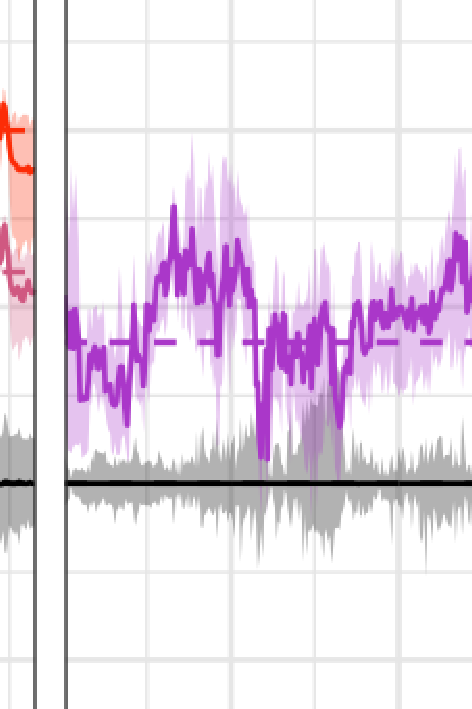
\includegraphics{/Users/aileneettinger/git/radcliffe/Analyses/figures/WarmingEffects_TimeSeries_SoilTemp1Mean_Deviation_NoPrecip.png}
 \caption{\textbf{Deviations in daily observed warming from mean control soil temperature for 12 study sites,} excluding data from plots that manipulated precipitation. We show soil, rather than above-ground, temperature, as this was the most frequently recorded temperature variable in the MC3E database. Solid lines show observed difference between warming treatment (colors) and control (black) plots, averaged across replicates and years; shading shows 95\% confidence intervals. Dashed lines represent target warming levels. (Note that the following sites had no explicit target temperature: exp06, exp11, exp12; in exp01, only the highest warming treatment had a target temperature; for these studies and treatments, we used their reported level of warming.) Two sites not shown here did not monitor soil temperature. Sites are ordered by low to high mean annual soil temperature (shown in the upper right corner of each panel). The heating type is listed in parentheses next to the site number (IR= infrared, soil= soil cables, air= forced air; con= constant wattage warming control). } %The number of temperature treatment levels vary from one (e.g. exp08, exp11) to nine (exp07 and exp10, which used an unreplicated regression design). Daily temperature values were obtained by averaging across years for each day of the year in each temperature treatment in each study. 
 \label{fig:effwarm}
 \end{figure}
 
 \begin{figure}[h!]
\centering

 \includegraphics[width=50mm]{/Users/aileneettinger/git/radcliffe/Analyses/figures/Box1Figure_captions.png} 
 %
 \caption*{} 
 
\label{fig:exps}
\end{figure}
 

 \begin{figure}[h]
 \centering
 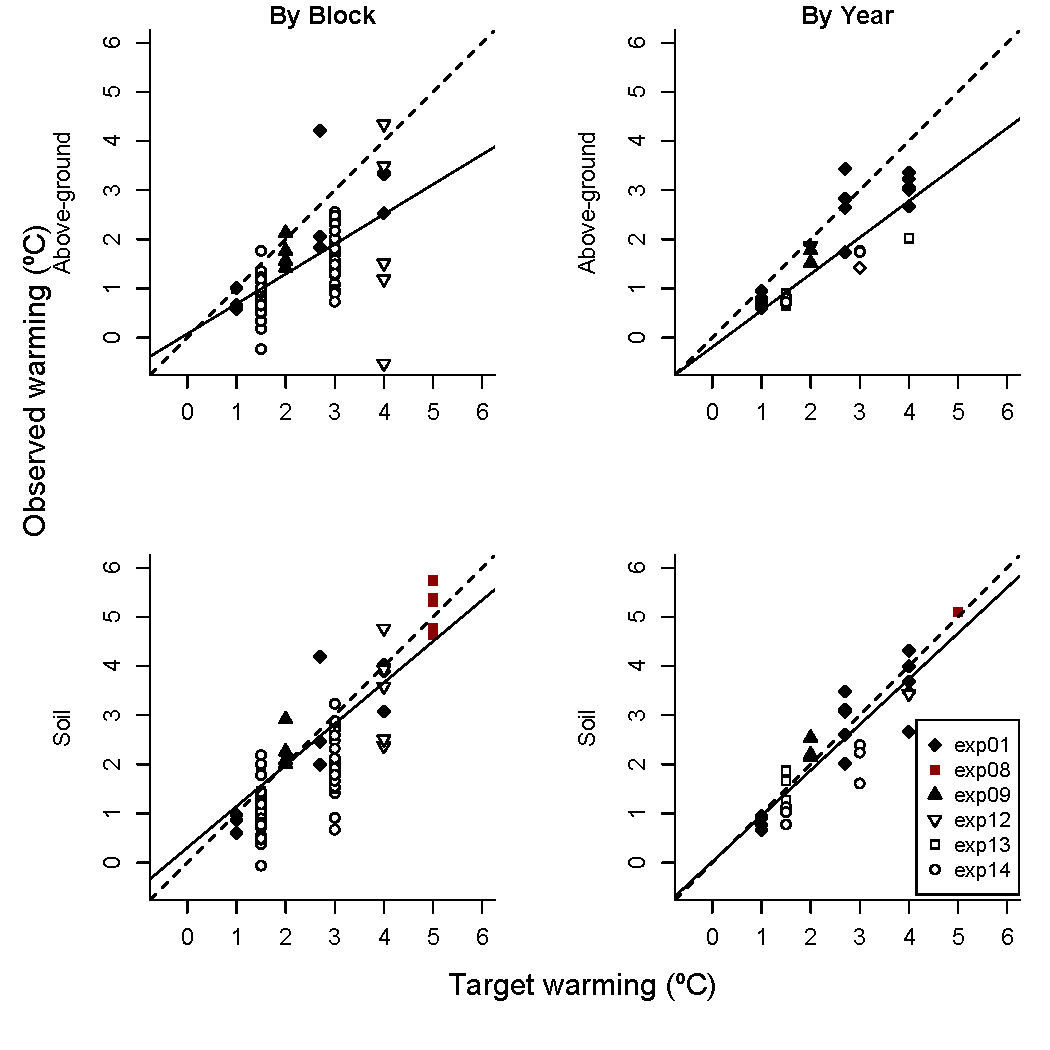
\includegraphics{/Users/aileneettinger/git/radcliffe/Analyses/figures/blockyearvar_target2.pdf} 
 \caption{\textbf{Observed warming over space and time, for above-ground and soil temperatures,} excluding data from plots that manipulated precipitation. Above-ground temperature includes air, canopy, and surface temperature. Points represent the difference between treatment and control plots by block (i.e., one data point per block) and by year (i.e., one data point per year). The solid line is the fitted relationship between observed and target warming and the dashed line shows when observed warming is exactly equal to target warming (1:1). Black symbols represent studies using infrared; red represents soil warming cables (only exp08); no studies with forced air heating used a blocked design. Open symbols represent constant wattage control and filled symbols represent feedback control. Note that the following studies had no explicit target temperature: exp06, exp11, exp12; for these studies, we used their reported level of warming. For exp01, only the treatment with the greatest warming had a target temperature. See Supplemental Materials (especially Tables S5 and S6) for details.}
 \label{fig:blockyear}
 \end{figure}

 \begin{figure}[h]
\centering
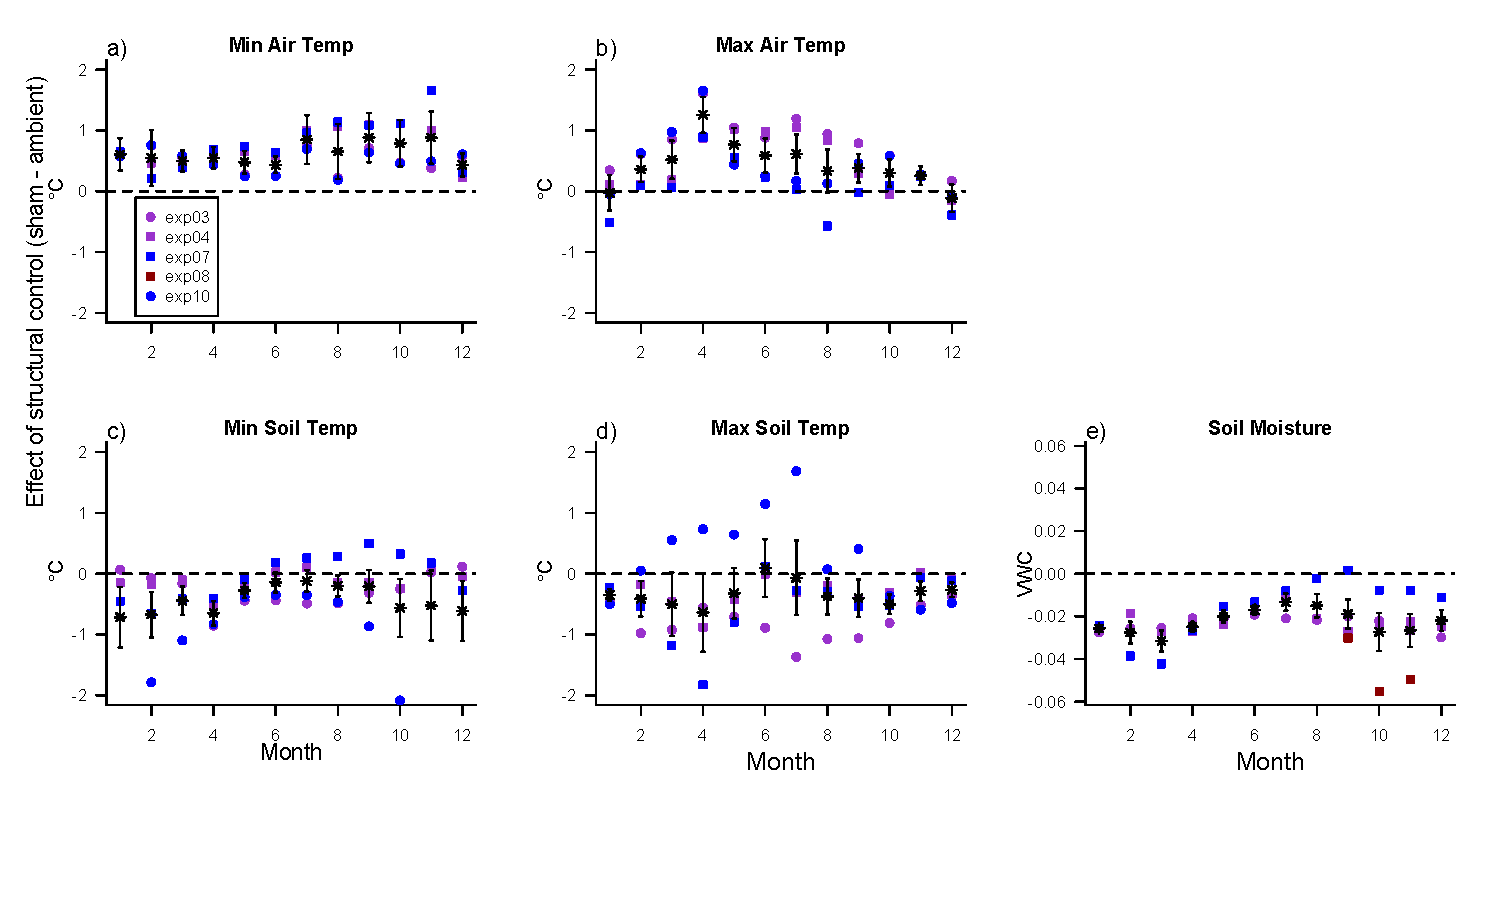
\includegraphics[height=100mm,width=180mm]{/Users/aileneettinger/git/radcliffe/Analyses/figures/ShamVSAmbient_all.pdf} 
 \caption{\textbf{Deviations in measured abiotic variables by month in structural controls compared to ambient controls} (i.e., with no control chambers or warming infrastructure in place). Above-ground temperatures (which include includes air, canopy, and surface temperatures) were higher (a,b), whereas soil temperature (c,d) and soil moisture (e) were lower in structural controls compared with ambient controls. We show overall (fixed) effects in black from monthly mixed-effects models; site-level random effects are shown by squares (for the three studies conducted at Harvard Forest in Massachusetts, USA) and circles (the two studies conducted at Duke Forest in North Carolina, USA). Colors vary by heating type: red represents soil warming cables, blue represents forced air; purple represents combined soil warming cables and forced air heating (no studies with infrared heating included both control types). All studies included used feedback warming control. See Supplemental Materials for details (Tables S8-S13). }
 \label{fig:shamamb}
 \end{figure}
\clearpage
 \begin{figure}[h!]
 \centering
 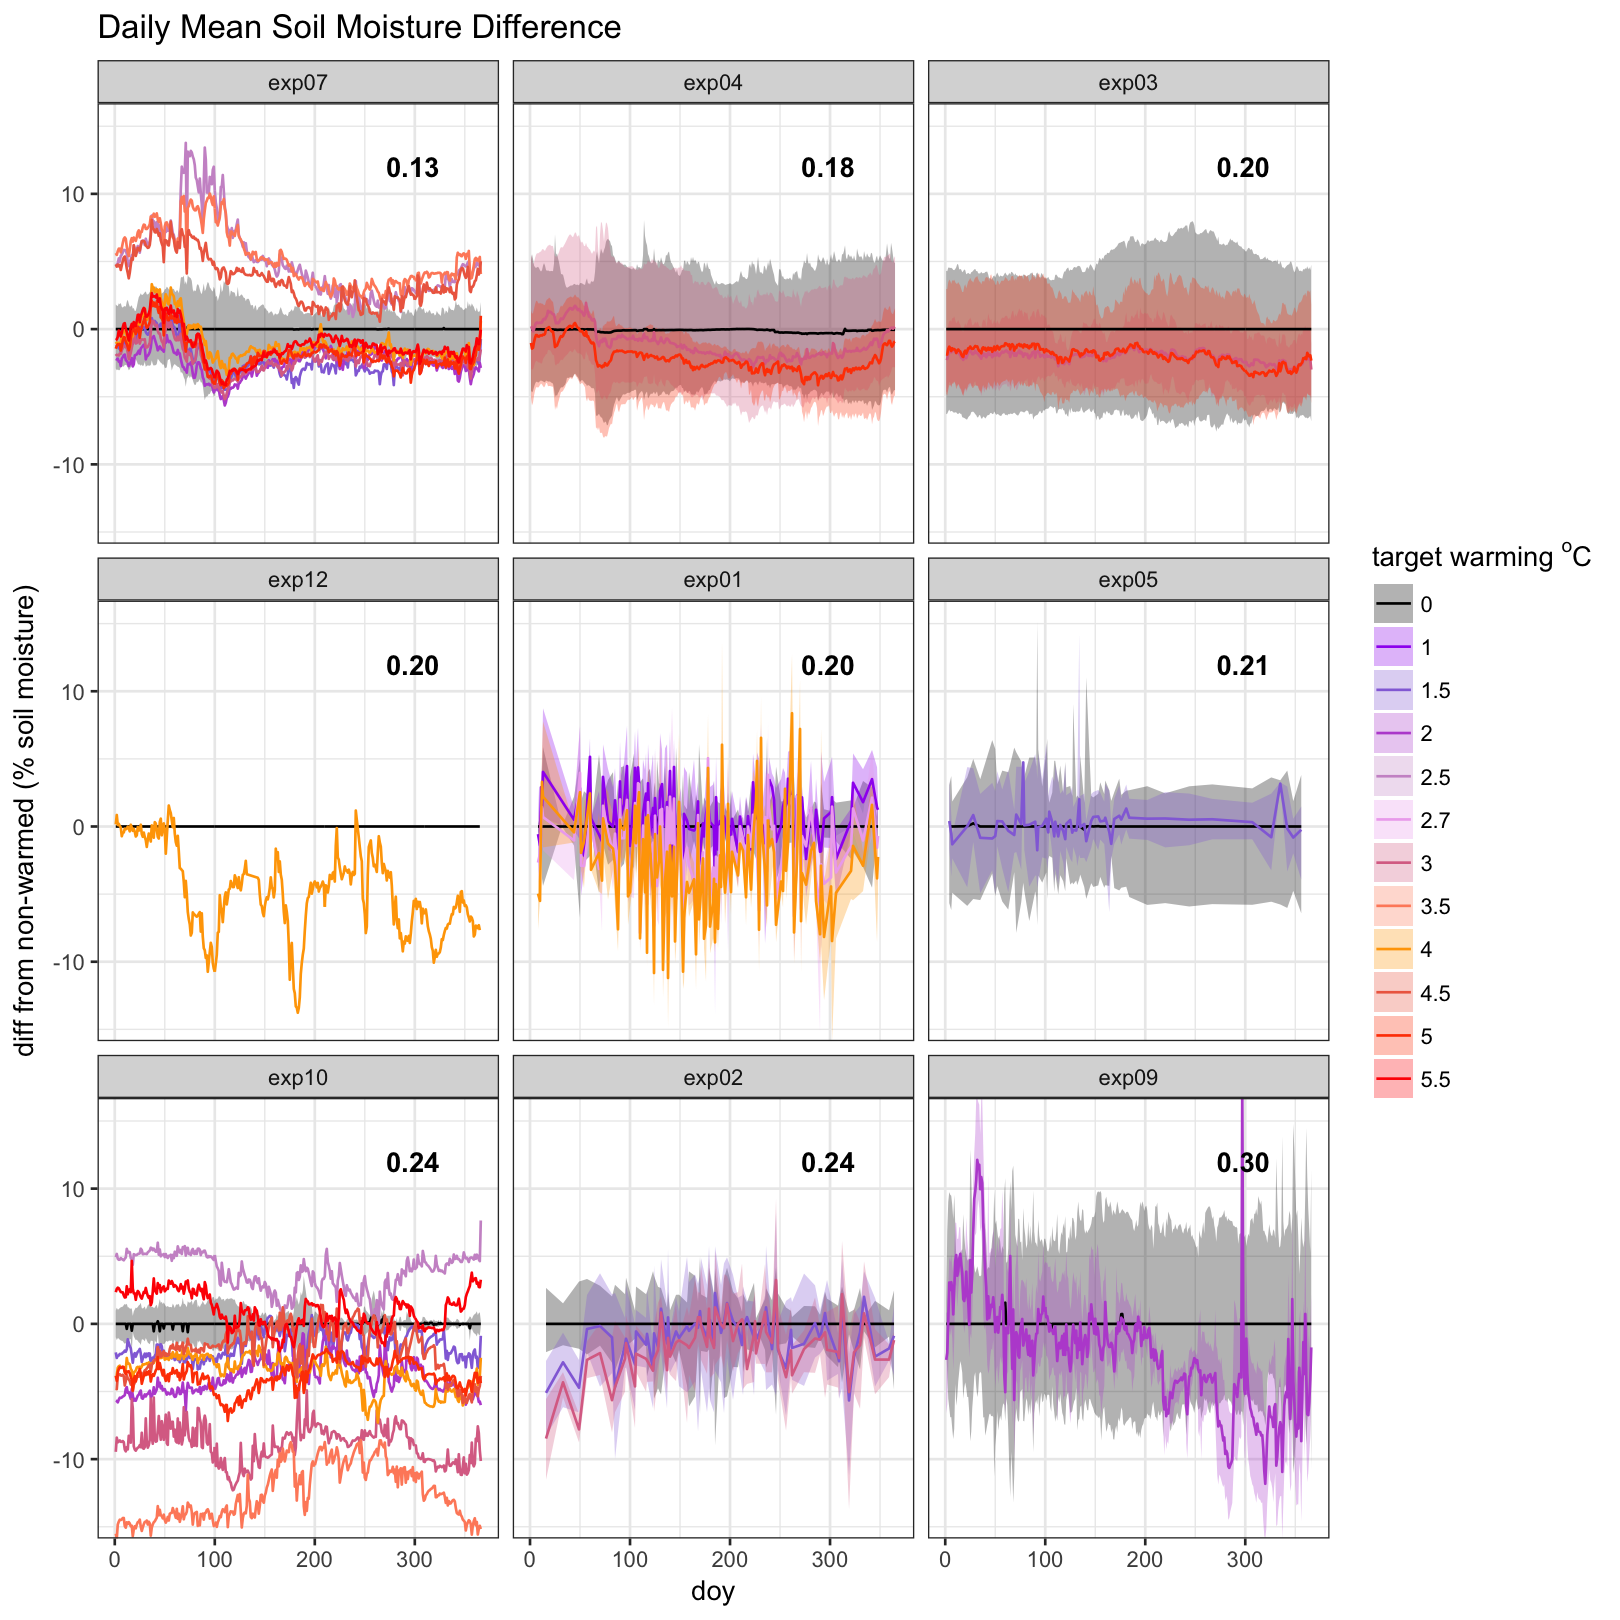
\includegraphics{/Users/aileneettinger/git/radcliffe/Analyses/figures/WarmingEffects_TimeSeries_SoilMoist_Deviation_NoPrecip.png} 
 \caption{\textbf{Deviations in daily observed soil moisture,} shown for the 11 study sites that continuously monitored soil moisture, excluding data from plots that manipulated precipitation. Black lines represent control plots, and colored lines represent warming treatments with various target warming levels (or reported warming, if there was no explicit target temperature). The number of temperature treatment levels vary from one (e.g., exp08, exp11) to nine (exp07 and exp10, which used an unreplicated regression design). Sites are ordered by low to high mean annual soil moisture (shown in the upper right corner of each plot). All experiments measured soil moisture in volumetric water content, as a percentage of the soil volume in the sample, scaled from 0 to 100; the absolute difference between treatment and control plots is shown. Heating type is listed in parentheses next to the site number: IR-con= infrared with constant wattage, IR-f= infrared with feedback control), soil= soil cables, air= forced air.}. 
 \label{fig:mois}
 \end{figure}
 \clearpage
 \begin{figure}[h!]
\centering
 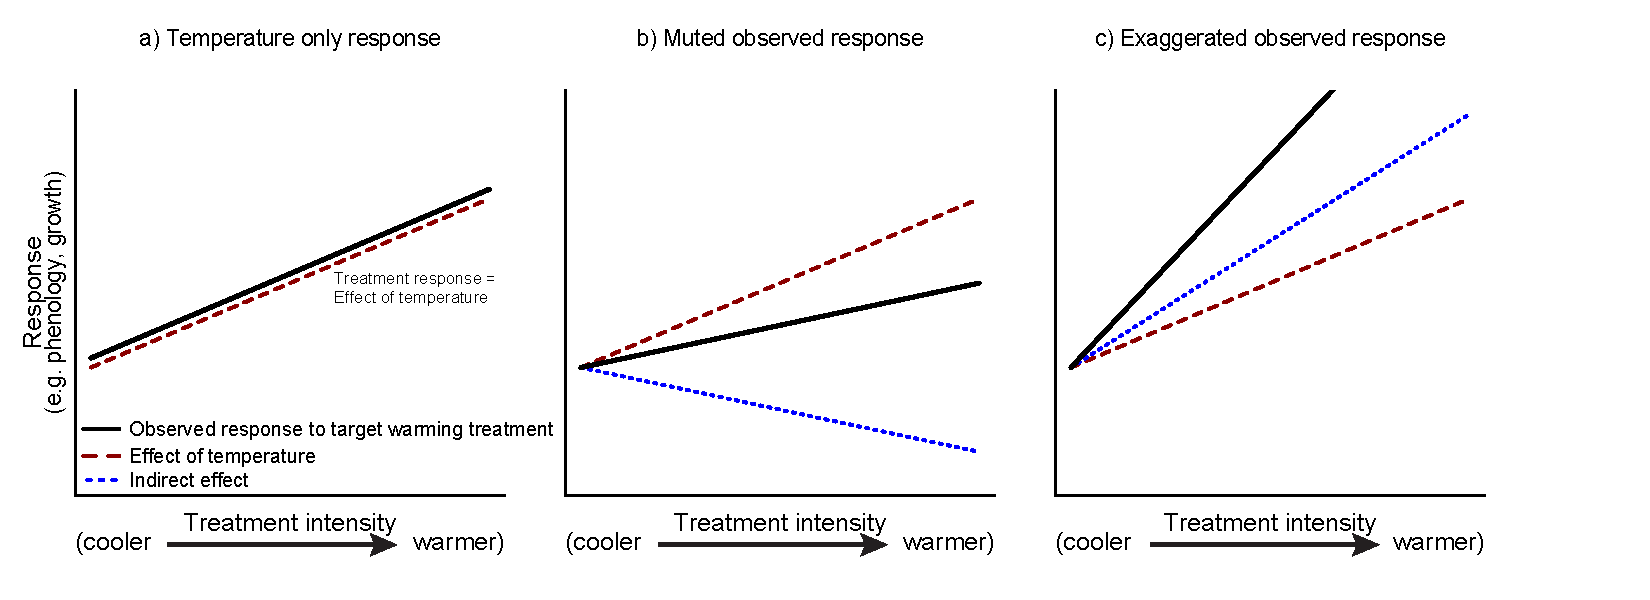
\includegraphics[height=70mm,width=200mm]{/Users/aileneettinger/git/radcliffe/Analyses/figures/DirIndWarmingEffects.pdf} 
 \caption{\textbf{Theoretical biological responses to experimental warming and their interpretation}. Direct responses to temperature alone (a) can be easily understood. Complications arise when biological responses are a mix of the direct temperature and indirect non-temperature effects of experimental warming. Then experimental warming may cause biological responses to be muted (b) or exaggerated (c). Quantifying, interpreting, and reporting these non-temperature effects in experiments is critical, and their presence is both a strength and a challenge of climate change experiments. They may represent ecologically realistic effects that might not have been predicted without the \emph{in situ} field experiment. Alternatively, they may represent artifacts that are unlikely to occur outside of an experimental context. Slopes of these example lines assume a linear response with additive direct and indirect effects. The relationship between these effects could be more complex (e.g., nonlinear; antagonistic, multiplicative, or otherwise interactive).} 
\label{fig:biolimp}
\end{figure}
\clearpage
\begin{figure}[h!]
\centering
 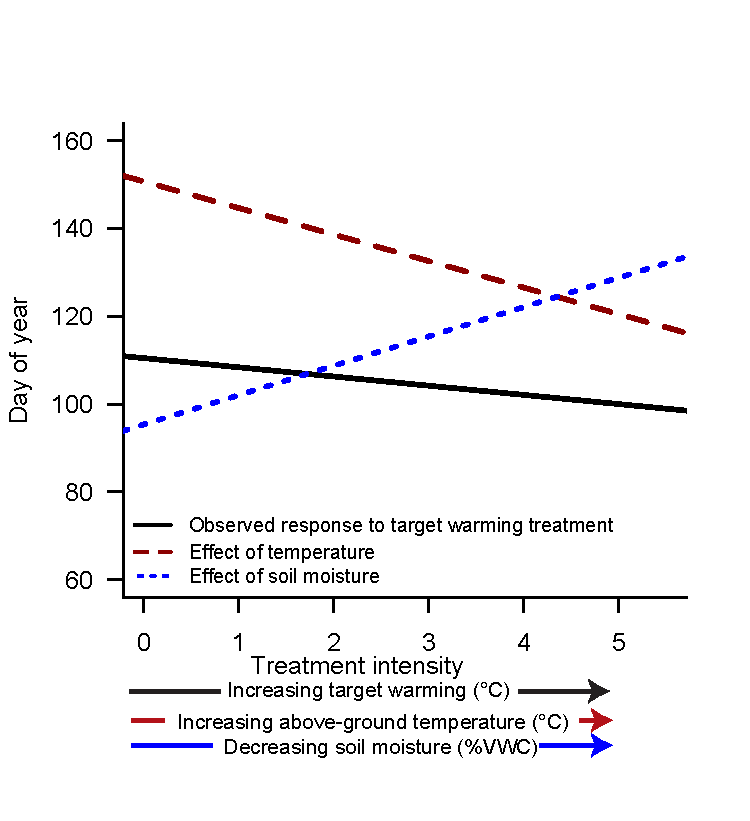
\includegraphics{/Users/aileneettinger/git/radcliffe/Analyses/figures/DirIndWarmingEffects_ExBBSM_reltemp.pdf} 
 %
 \caption{\textbf{Observed response of budburst day of year to experimental climate change} is an example of a muted response: the observed response to increasing treatment intensity (i.e., the coefficient of a model fit with only target [or reported, if there was no explicit target] temperature as the explanatory variable, black line; units for x-axis are \degree C of target warming) suggests a weaker temperature sensitivity than the effect of temperature in a more biologically accurate (and better-fitting) model that includes both measured above-ground temperature (dashed red line, for which x-axis units are \degree C of measured temperature) and soil moisture (dotted blue line, for which x-axis units are \% VWC, decreasing from left to right in conjunction with warming intensity), as well as their interaction. Analysis includes all studies that monitored budburst and measured soil moisture and above-ground temperature (exp01, exp03, exp04, exp07, exp10); structural control data were used for this analysis (ambient controls were excluded from those studies that contained both). See Supplemental Materials, especially Tables S17 \& S18, for additional details.} 
 
\label{fig:phen}
\end{figure}
\clearpage
\section* {Box 1: Different methods for achieving warming.}
Active-warming experiments may differ both in the way that they achieve warming (``warming type" in Table S1), and the way that warming is controlled (``warming control" in Table S1). There are three warming types used by studies in the MC3E database. These are infrared (n=9), an open-air method in which infrared heaters are mounted above the ground; forced air (n=3), in which air is heated and then pumped through an airflow system into a chamber; and soil warming (n=1), a chamber-less method in which soil is heated with buried electric resistance cable. Two additional studies in the database used combined forced air in chambers and soil warming. Warming is controlled by either constant wattage, in which an unvarying energy output is used, or by feedback control, in which energy outputs are linked to a thermometer and varied depending on the measured temperature in plots, in order to maintain consistent warming levels. 
\par In this paper, we describe complications and non-temperature effects associated with active warming experiments, across these divergent warming methodologies. Some of the non-temperature effects described may be more likely to occur with particular methods than others. Alterations to airflow, for example, may be most dramatic with methods employing chambers. Plot shading and precipitation interference are likely to occur in chamber and infrared techniques, which both involve above-ground infrastructure, and less likely in methods that only warm from the soil. The biological impacts of such effects may be further enhanced or muted based on site characteristics (e.g., if a site is already heavily shaded, impacts from infrastructure shading may be lower).
\par Table \ref{tab:warmtech} highlights that there may be differences in non-temperature effects across these different warming methodologies. In the MC3E database, sample sizes within each warming and control type were quite low, so we were unable to statistically distinguish differences in non-temperature effects across the different methods in all analyses. For example, the constant wattage control studies have greater average variation (2.2 \degree C variation on average for constant versus 1.1 \degree C variation for feedback), but this difference is not significant (p=0.21). We note that the studies showing both the greatest and least variation employed constant wattage (greatest: plots in exp12, with target warming of 4.0 \degree C, varied by as much as 4.87 \degree C on average; least: plots in exp13 with 1.5 \degree C of target warming, varied by 0.03 \degree C per \degree C of target warming). These results are not conclusive, because our sample size is quite low (n=3 studies for constant and n=2 studies for feedback studies with blocked designs).
\par We expect that the list of non-temperature effects in Table \ref{tab:warmtech} is not exhaustive, but represents what we can document here or has been documented previously. We recommend additional detailed studies of these, and other, effects across warming designs. This will allow future researchers to more fully evaluate the challenges and opportunities of each method, and select an experimental approach well-suited to their particularly research focus.

\section* {Box 2: Recommendations for future climate change experiments} 
\begin{enumerate}
\item\textit{Collect and analyze plot-level climate data.} This includes analyzing and interpreting minimum and maximum values, as well as variance and critical thresholds \citep[e.g., the number and duration of freeze-thaw events and accumulated chilling hours,][]{mcdaniel2014,vasseur2014}. We suggest saving the raw data from data loggers (often collected at hourly or higher resolution) to allow quantification of variance (and other summaries) at different temporal resolutions. In assessing which frequency of measurements is most appropriate for analyses (e.g., hourly, twice daily), it is critical to consider the chronobiology of the event and organisms of interest. For ants, this might mean that temperatures be monitored every minute \citep{shavit2017}; for bacteria, even more frequently. 
\item\textit{Analyze measured climate variables rather than targets}. There can be substantial variation in the effects of warming and precipitation treatments among plots and across time (Figure \ref{fig:blockyear}). Analyzing measured climate will allow much more in-depth understanding of the drivers and biological effects of variation in temperature and moisture.
\item\textit{Publish high quality, usable data and metadata}. Given that climate manipulations are logistically challenging and expensive \citep{aronson2009}, and that they often produce a large volume of fine-scale climate data, good curation and data sharing will ensure wider use and deeper understanding of these valuable data. When studying biological implications of a global challenge as large as climate change, progress will come from designing and reporting experiments in ways that facilitate an eventual global data set. Researchers should also be explicit in their warming design (e.g., infrared heating with feedback control or forced air heating with constant wattage) to aid future analyses of the performance of different designs, across sites and over time (Box 1, Table \ref{tab:warmtech}).  
\item\textit{Include both structural and ambient controls} and collect, use, and report microclimate and biological data within them. Fewer than half of the studies in our MC3E database reported microclimate data from these two control types (6 out of 15 studies); however, all experiments that did include both control types showed significant effects of infrastructure (Figure \ref{fig:shamamb}).
\item\textit{Design relevant manipulations} by consulting observational records and forecasts, including seasonal and annual variation in projected warming. When it is not possible or desirable to match anticipated changes in climate, studies should report how imposed treatments compare to projected changes and past observations \citep[e.g.,][]{hoover2014, zhu2016}. In addition, if continuous treatments are not applied throughout the study, we recommend reporting the seasonality and timing of treatments and monitoring the climate throughout the year.

\item\textit{Maximize the duration of climate change experiments} by running some experiments for as long as possible, since the magnitude of climate change treatments can vary considerably among years (Figure \ref{fig:blockyear}). In addition, long-term responses of individuals and populations can differ from transient responses \citep{saleska2002,franklin1989,giasson2013,harte2015}. We were able to acquire data extending for $\geq$5 years for only one study in the MC3E database (exp01), restricting our ability to investigate the effect of study length on experimental climate change. %Well-designed and well-supported longer warming experiments will allow investigation of how inter-annual variations interact with climate change treatments, particularly when combined with observational studies and modeling \citep{luo2011}.
\item\textit{Conduct syntheses across studies}. As more detailed data are published from experimental climate change studies in divergent ecosystems and warming types, meta-analyses will advance our understanding of the ways that warming affects microclimate and biotic interactions. For example, it would be useful to compare microclimate data among studies using infrared warming applied with constant wattage versus infrared warming that varies energy inputs based on measured temperatures (Box 1). 

\end{enumerate}

\bibliography{/Users/aileneettinger/citations/Bibtex/mylibrary}

%%%%%%%%%%%%%%%%%%%%%%%%%%%%%%%%%%%%%%%%
\end{document}
%%%%%%%%%%%%%%%%%%%%%%%%%%%%%%%%%%%%%%%%
